\chapter{Síntesis de Sonidos mediante Modelos Físicos}

\section{Introducción}
Se utilizó el modelo de Karplus-Strong para sintetizar el sonido de instrumentos de cuerda percutida u otros tipos de percusión. Este algoritmo, creado por Kevin Karplus y Alexander Strong en 1983 para sintetizar sonidos con pocos recursos y a tiempo real.

En este trabajo se analizaron el modelo básico para la síntesis de cuerdas percutidas y el modelo modificado para la síntesis de instrumentos de percusión.

\section{Modelo Conceptual}

En principio se trata de un sistema linear excitado con una secuencia aleatoria de longitud finita. Consiste de una línea de retarde de L muestras retroalimentadas mediante un filtro. Este se puede ver en la figura \ref{fig:KS_model}.

\begin{figure}[ht]
    \centering
    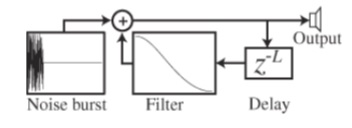
\includegraphics{res/ks_concept.jpg}
    \caption{Diagrama Conceptual del Modelo de Karplus-Strong}
    \label{fig:KS_model}
\end{figure}

La línea de retardo simula cómo los distintos armónicos de una nota recorren la línea, se atenúan y decaen en el tiempo. Se suele utilizar un filtro pasa-bajos para atenuar más rápidamente los armónicos de más altas frecuencias. Nótese que la longitud de la secuencia de entrada debe tener una longitud L.

La primera etapa de este modelo promedia dos muestras consecutivas. Este proceso puede describirse matemáticamente como la ecuación \eqref{eq:KS_avg}.

\begin{equation}
    Y_t = 0.5\times \left(Y_{t-p}+Y_{t-p-1}\right)
    \label{eq:KS_avg}
\end{equation}

Resulta que este promediamiento produce una onda que decae más lentamente en el tiempo. El onda generada por este algoritmo corresponde a un tono con período $L + 0.5$ muestras (que corresponde a una frecuencia de $f_s / (L+0.5)$) y suena más cercanamente al sonido de una cuerda punteada.

Independientemente de las condiciones iniciales del sistema, el espectro decaerá a un tono puro, y eventualmente, a una constante (el silencio).

\begin{equation}
    Y_t = 
    \begin{cases}
        +A  &   \text{probabilidad 0.5}\\
        -A  &   \text{probabilidad 0.5}
    \end{cases}
    \qquad  \text{para} -L\leq t \leq 0
\end{equation}

